\section{Rangga Putra Ramdhani}
\subsection{Buatlah librari fungsi (library dengan nama NPM bar.py) untuk plot dengan jumlah subplot adalah NPM mod 3 + 2}
\lstinputlisting[caption = fungsi bar., firstline=11, lastline=38]{src/6/Praktek/1174056/1174056_bar.py}
\begin{figure}[H]
	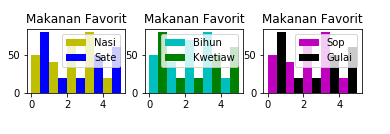
\includegraphics[width=9cm]{figures/6/Praktek/1174056/bar.png}
	\caption{Hasil dari fungsi bar.}
	\centering
\end{figure}

\subsection{Buatlah librari fungsi (library dengan nama NPM scatter.py) untuk plot dengan jumlah subplot NPM mod 3 + 2}
\lstinputlisting[caption = fungsi scatter., firstline=12, lastline=48]{src/6/Praktek/1174056/1174056_scatter.py}
\begin{figure}[H]
	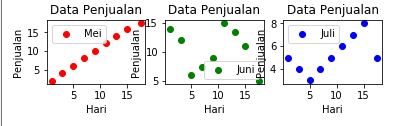
\includegraphics[width=9cm]{figures/6/Praktek/1174056/scatter.png}
	\caption{Hasil dari fungsi scatter.}
	\centering
\end{figure}

\subsection{Buatlah librari fungsi (library dengan nama NPM pie.py) untuk plot dengan jumlah subplot NPM mod 3 + 2}
\lstinputlisting[caption = fungsi pie., firstline=11, lastline=64]{src/6/Praktek/1174056/1174056_pie.py}
\begin{figure}[H]
	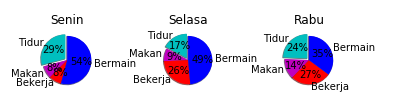
\includegraphics[width=9cm]{figures/6/Praktek/1174056/pie.png}
	\caption{Hasil dari fungsi pie.}
	\centering
\end{figure}

\subsection{Buatlah librari fungsi (library dengan nama NPM plot.py) untuk plot dengan jumlah subplot NPM mod 3 + 2}
\lstinputlisting[caption = fungsi plot., firstline=8, lastline=30]{src/6/Praktek/1174056/1174056_plot.py}
\begin{figure}[H]
	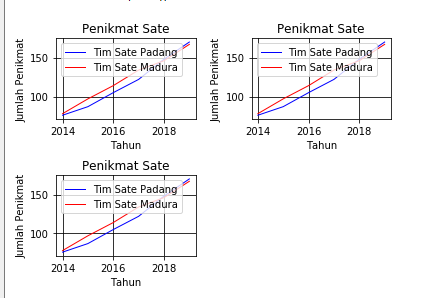
\includegraphics[width=9cm]{figures/6/Praktek/1174056/plot.png}
	\caption{Hasil dari fungsi plot.}
	\centering
\end{figure}

\subsection{Screenshoot main}
\begin{figure}[H]
	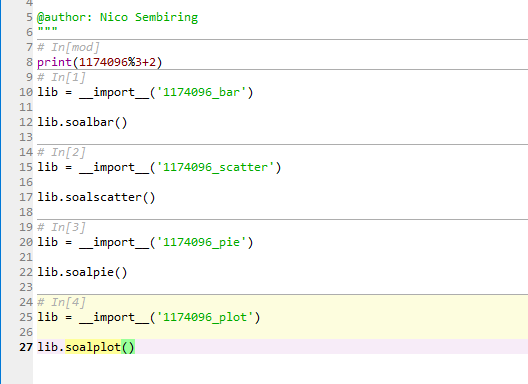
\includegraphics[width=9cm]{figures/6/Praktek/1174056/kodinganmain.png}
	\caption{kodingan main.}
	\centering
\end{figure}

\subsection{Screenshoot mod}
\begin{figure}[H]
	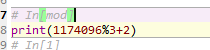
\includegraphics[width=9cm]{figures/6/Praktek/1174056/kodingmod.png}
	\caption{kodingan mod.}
	\centering
\end{figure}

\begin{figure}[H]
	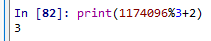
\includegraphics[width=9cm]{figures/6/Praktek/1174056/hasilmod.png}
	\caption{hasil mod.}
	\centering
\end{figure}

\subsection{Pengecekan Plagiarisme Praktek}
\begin{figure}[H]
	\includegraphics[width=9cm]{figures/6/Praktek/1174056/Plagiatpraktek.png}
	\centering
\end{figure}

\subsection{Ketrampilan Penanganan Error}
\textbf{Tuliskan peringatan error yang didapat dari mengerjakan praktek ketiga ini, dan jelaskan cara penanganan error tersebut. dan Buatlah satu fungsi yang menggunakan gunakan try except untuk menanggulangi error tersebut}

Peringatan error yang saya temui pada praktek Chapter 6 ini, adalah:
\begin{itemize}
	\item Name Error
	NameError adalah exception yang terjadi ketika kode melakukan eksekusi terhadap local name atau global name yang tidak terdefinisi oleh perangkat. Solusi yang dapat dilakukan adalah dengan memastikan variabel atau fungsi yang dipanggil ada atau tidak salah ketik.
	
	\item Syntax Errors
	Syntax Errors adalah suatu keadaan saat  terjadi kesalahan penulisan pada kode python. Cara memperbaikinya adalah dengan memperbaiki penulisan kode yang salah.
	
	\item Type Error
	TypeError adalah exception yang terjadi pada saat dilakukannya eksekusi terhadap suatu operasi atau fungsi dengan type object yang tidak sesuai. Cara yang dilakukan untuk mengatasinya error ini adalah mengkoversi varibelnya sesuai dengan tipe data yang akan digunakan.
\end{itemize}

\textbf{Penanggulangan Error menggunakan Try Except}
\lstinputlisting[caption = Penanggulangan error menggunakan Try Except., firstline=8, lastline=25]{src/6/Praktek/1174056/1174056_error.py}

\subsection{Pengecekan Plagiarisme Penanganan Error}
\begin{figure}[H]
	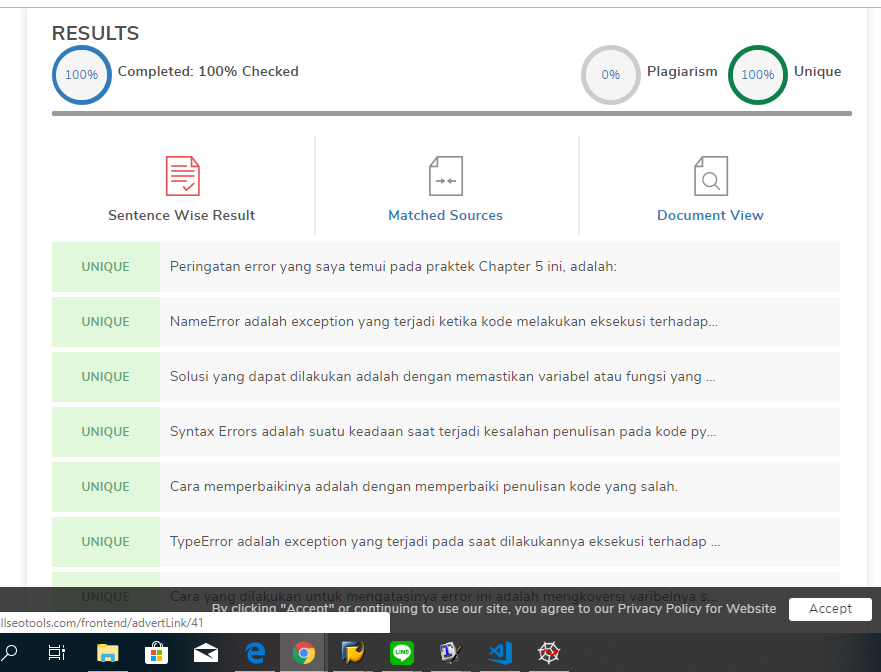
\includegraphics[width=9cm]{figures/6/Praktek/1174056/Plagiarismeerror.png}
	\centering
\end{figure}
